% Created 2023-01-26 Thu 18:14
% Intended LaTeX compiler: lualatex
\documentclass[11pt]{article}
\usepackage{graphicx}
\usepackage{longtable}
\usepackage{wrapfig}
\usepackage{rotating}
\usepackage[normalem]{ulem}
\usepackage{amsmath}
\usepackage{amssymb}
\usepackage{capt-of}
\usepackage{hyperref}
\usepackage[margin=0.5in]{geometry}
\usepackage{minted}
\author{David Lewis}
\date{1/26/2023}
\title{Lec 6: Classroom activity}
\hypersetup{
 pdfauthor={David Lewis},
 pdftitle={Lec 6: Classroom activity},
 pdfkeywords={},
 pdfsubject={},
 pdfcreator={Emacs 28.2 (Org mode 9.6)}, 
 pdflang={English}}
\begin{document}

\maketitle
\section*{1.}
\label{sec:org768e5ad}
\subsection*{a.}
\label{sec:orge6d7b7a}
\begin{center}
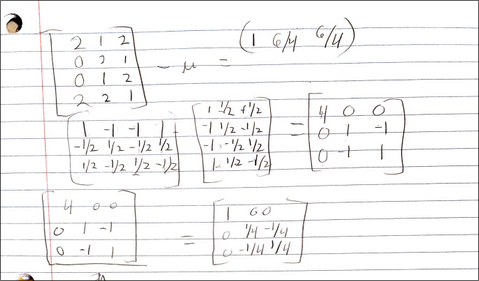
\includegraphics[width=8cm]{a.png}
\end{center}
\begin{itemize}
\item \(\begin{bmatrix} 1 & 0 & 0 \\
                    0 & 0.25 & -0.25 \\
                    0 & -0.25 & 0.25 \end{bmatrix}\)
\end{itemize}
\subsection*{b.}
\label{sec:orgf6d1829}
\begin{itemize}
\item \(\begin{bmatrix} 1 & 0 & 0 \\
                    0 & 0.25 & -0.25 \\
                    0 & -0.25 & 0.25 \end{bmatrix} \begin{bmatrix}1 \\ 0 \\ 0
  \end{bmatrix} = \begin{bmatrix}1 \\ 0 \\ 0
  \end{bmatrix}\)
\item normalized is \(\frac{ \begin{bmatrix}1 \\ 0 \\ 0
  \end{bmatrix}} {1}\)
\item first eigenvector is \(\begin{bmatrix}1 \\ 0 \\ 0
  \end{bmatrix}\)
\item first eigenvalue is 1
\end{itemize}
\subsection*{c.}
\label{sec:orgcbbbbaf}
\begin{itemize}
\item \(B = A - \lambda vv^T = \(\begin{bmatrix} 1 & 0 & 0 \\
                    0 & 0.25 & -0.25 \\
                    0 & -0.25 & 0.25 \end{bmatrix} - \(\begin{bmatrix} 1 & 0 & 0 \\
                    0 & 0 & 0 \\
                    0 & 0 & 0 \end{bmatrix} = \(\begin{bmatrix} 0 & 0 & 0 \\
                    0 & 0.25 & -0.25 \\
                    0 & -0.25 & 0.25 \end{bmatrix}\)
\end{itemize}

\subsection*{d.}
\label{sec:org626e871}
\begin{center}
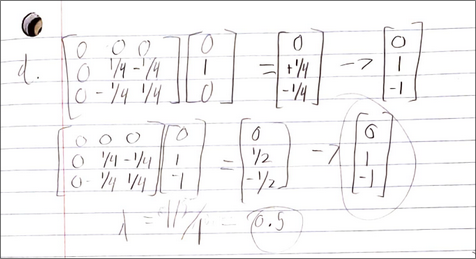
\includegraphics[width=8cm]{d.png}
\end{center}
\subsection*{e and f.}
\label{sec:orge67ab52}
\begin{center}
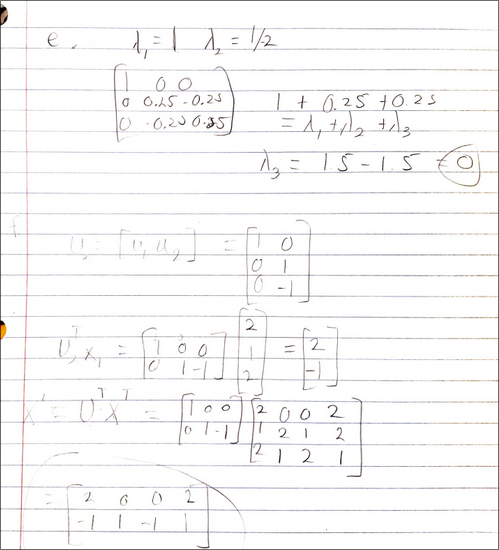
\includegraphics[width=8cm]{ef.png}
\end{center}

\section*{2.}
\label{sec:orgedd4c9e}
\subsection*{a.}
\label{sec:orgb1ebb68}
\(\begin{bmatrix} 4.26 & 0.323 & 0.323 \\
3.14 & 0.238 & 0.561 \\
2.0 & 0.152 & 0.713 \\
1.92 & 0.146 & 0.859 \\
1.03 & 0.078 & 0.936 \\
0.84 & 0.064 & 1.0 \end{bmatrix}\)
\subsection*{b.}
\label{sec:org32a33c6}
The first two principal directions correspond to the first two eigenvalues
(largest 2). The variance from these two directions is the sum of these
eigenvalues \(4.26 + 3.14 = 7.4\)
\subsection*{c.}
\label{sec:orge50115a}
The number of eigenvectors needed to explain at least 80\% of the variance is 4.
This is shown in the table above by the cumulative proportion of variance
captured, which is 85.9\% at 4 eigenvalues.
\end{document}
